\documentclass[12pt,a4paper]{extarticle}
\usepackage{../templates/preamble}

\renewcommand{\typeofnum}{2}
\renewcommand{\papertheme}{Работа с текстом.}

\begin{document}
\input{../templates/titlepage.tex}
\setcounter{page}{2}
\tableofcontents
\newpage

% document %
\section{Исходная формулировка задания}
В заданном тексте, содержащей синтаксически корректное выражение на С++. В явном объявлении
массивов выделить имена массивов и определить, являются ли они одномерными. Поиск должен производится
блочным представлением текста.

\section{Определение неясностей}
Размеры блока задаются статически в отдельном заголовочном файле.

\section{Контрольный пример}

\begin{tabularx}{\textwidth}{|>{\ttfamily\footnotesize}X|}
    \hline
    \multicolumn{1}{|>{\centering\arraybackslash}X|}{Ввод} \\ \hline
    \lstinputlisting{../../tasks/2/in.txt} \\ \hline
    \multicolumn{1}{|>{\centering\arraybackslash}X|}{Вывод} \\ \hline
    Блок 3:0 считан\par
    = \{2, \{ найден массив: array | одномерный \}\par
    ; \{ найден массив: list | многомерный \}\par
    [] =  \{ найден массив: massiv | одномерный \} \\ \hline
\end{tabularx}

% \section{Ограничения, обусловленные вычислительным устройством}

\section{Формат файлов}
Входные и выходные файлы для маркерного представления должны иметь следующие форматы:

\begin{xltabular}{\textwidth}{|>{\ttfamily\footnotesize}X|}
    \hline
    \multicolumn{1}{|>{\centering\arraybackslash}X|}{Входные файлы} \\ \hline
    [синтаксически корректный блок кода на C++] \\ \hline

    \multicolumn{1}{|>{\centering\arraybackslash}X|}{Выходные файлы} \\ \hline
    Блок X:Y считан \par
    ccc \par
    ccc \{ найден ответ: name | \{одномерный, многомерный\} \}\par
    ccc \par
     \\ \hline
\end{xltabular}

\section{Реализация ввода/вывода}
\begin{xltabular}{\textwidth}{|h|s|s|}
    \hline
    \multicolumn{1}{|h|}{Библиотека} &
    \multicolumn{1}{s|}{Ввод} &
    \multicolumn{1}{s|}{Вывод}\\ \hline
    iostream & cin > > & cout < < \\ \hline
    fstream & istream & ostream \\ \hline
\end{xltabular}

\section{Внутреннее представление данных}
\begin{xltabular}{\textwidth}{|
>{\hsize=.2\hsize\centering\arraybackslash\ttfamily\bfseries}X|
>{\hsize=.2\hsize\centering\arraybackslash\itshape}X|
>{\hsize=.6\hsize\centering\arraybackslash}X|
}
\hline
\multicolumn{1}{|>{\hsize=.2\hsize\centering\arraybackslash}X}{Имя переменной} &
\multicolumn{1}{|>{\hsize=.2\hsize\centering\arraybackslash}X}{Тип} &
\multicolumn{1}{|>{\hsize=.6\hsize\centering\arraybackslash}X|}{Описание} \\ \hline
counts & chunk\_count & Разбиение блока на блоки \\ \hline
in & ifstream & Входной файл \\ \hline
out & ofstream & Выходной файл \\ \hline
pivots & txtPivots & Краи строк текста \\ \hline
chunk & chunkL & Блок текста \\ \hline
mid\_chunk & readState & Статус прочтения строки блоков \\ \hline
result & resultStates & Сохранённые результаты обработки \\ \hline

\end{xltabular}
Структура {\ttfamily\bfseries chunk\_count} (из {\ttfamily chunkL.hpp}):
\begin{xltabular}
    {\textwidth}{|
    >{\hsize=.2\hsize\centering\arraybackslash\ttfamily\bfseries}X|
    >{\hsize=.2\hsize\centering\arraybackslash\itshape}X|
    >{\hsize=.6\hsize\centering\arraybackslash}X|
    }
    \hline
    \multicolumn{1}{|>{\hsize=.2\hsize\centering\arraybackslash}X}{Имя аргумента} &
    \multicolumn{1}{|>{\hsize=.2\hsize\centering\arraybackslash}X}{Тип} &
    \multicolumn{1}{|>{\hsize=.6\hsize\centering\arraybackslash}X|}{Описание} \\ \hline
% \input{../templates/datatype.tex}
w & unsigned & Количество блоков по x \\ \hline
h & unsigned & Количество блоков по h \\ \hline
\end{xltabular}

Класс {\ttfamily\bfseries chunkL} (из {\ttfamily chunkL.hpp}):
\begin{xltabular}{\textwidth}{|
>{\hsize=.2\hsize\centering\arraybackslash\ttfamily\bfseries}X|
>{\hsize=.1\hsize\centering\arraybackslash\itshape}X|
>{\hsize=.7\hsize\centering\arraybackslash}X|}
\hline
\multicolumn{1}{|>{\hsize=.2\hsize\centering\arraybackslash}X}{Имя аргумента} &
\multicolumn{1}{|>{\hsize=.1\hsize\centering\arraybackslash}X}{Тип} &
\multicolumn{1}{|>{\hsize=.7\hsize\centering\arraybackslash}X|}{Описание} \\ \hline
lines & strL* & Строки блока \\ \hline
lines\_c & unsigned & Длина блока \\ \hline
\end{xltabular}

Класс {\ttfamily\bfseries strL} (из {\ttfamily strL.hpp}):
\begin{xltabular}{\textwidth}{|
>{\hsize=.2\hsize\centering\arraybackslash\ttfamily\bfseries}X|
>{\hsize=.1\hsize\centering\arraybackslash\itshape}X|
>{\hsize=.7\hsize\centering\arraybackslash}X|}
\hline
\multicolumn{1}{|>{\hsize=.2\hsize\centering\arraybackslash}X}{Имя аргумента} &
\multicolumn{1}{|>{\hsize=.1\hsize\centering\arraybackslash}X}{Тип} &
\multicolumn{1}{|>{\hsize=.7\hsize\centering\arraybackslash}X|}{Описание} \\ \hline
chars & char* & Символы строки \\ \hline
chars\_c & unsigned & Длина строки \\ \hline
offset & int & Оффсет чтения с файла \\ \hline
\end{xltabular}

Класс {\ttfamily\bfseries txtPivots} (из {\ttfamily files.hpp}):
\begin{xltabular}{\textwidth}{|
>{\hsize=.2\hsize\centering\arraybackslash\ttfamily\bfseries}X|
>{\hsize=.1\hsize\centering\arraybackslash\itshape}X|
>{\hsize=.7\hsize\centering\arraybackslash}X|}
\hline
\multicolumn{1}{|>{\hsize=.2\hsize\centering\arraybackslash}X}{Имя аргумента} &
\multicolumn{1}{|>{\hsize=.1\hsize\centering\arraybackslash}X}{Тип} &
\multicolumn{1}{|>{\hsize=.7\hsize\centering\arraybackslash}X|}{Описание} \\ \hline
starts & int* & Индексы чтения начала строк \\ \hline
ends & int* & Индексы чтения конца строк \\ \hline
pivots\_c & unsigned & Длина текста \\ \hline
\end{xltabular}

Структура {\ttfamily\bfseries lineState} (из {\ttfamily readState.hpp}):
\begin{xltabular}{\textwidth}{|
>{\hsize=.2\hsize\centering\arraybackslash\ttfamily\bfseries}X|
>{\hsize=.1\hsize\centering\arraybackslash\itshape}X|
>{\hsize=.7\hsize\centering\arraybackslash}X|}
\hline
\multicolumn{1}{|>{\hsize=.2\hsize\centering\arraybackslash}X}{Имя аргумента} &
\multicolumn{1}{|>{\hsize=.1\hsize\centering\arraybackslash}X}{Тип} &
\multicolumn{1}{|>{\hsize=.7\hsize\centering\arraybackslash}X|}{Описание} \\ \hline
state & State & Текущий статус чтения \\ \hline
name\_start & int & Индекс чтения начала имени \\ \hline
name\_ends & int & Инкриминированный индекс чтения конца имени \\ \hline
opened\_bracket & int & Индекс чтения начала скобок \\ \hline
opened\_bracket & int & Инкриминированный индекс чтения конца скобок \\ \hline
\end{xltabular}

Структура {\ttfamily\bfseries readState} (из {\ttfamily readState.hpp}):
\begin{xltabular}{\textwidth}{|
>{\hsize=.2\hsize\centering\arraybackslash\ttfamily\bfseries}X|
>{\hsize=.1\hsize\centering\arraybackslash\itshape}X|
>{\hsize=.7\hsize\centering\arraybackslash}X|}
\hline
\multicolumn{1}{|>{\hsize=.2\hsize\centering\arraybackslash}X}{Имя аргумента} &
\multicolumn{1}{|>{\hsize=.1\hsize\centering\arraybackslash}X}{Тип} &
\multicolumn{1}{|>{\hsize=.7\hsize\centering\arraybackslash}X|}{Описание} \\ \hline
l & lineState[H] & Список статусов чтения длинной высоты блока \\ \hline
\end{xltabular}

Класс {\ttfamily\bfseries resultStates} (из {\ttfamily readState.hpp}):
\begin{xltabular}{\textwidth}{|
>{\hsize=.2\hsize\centering\arraybackslash\ttfamily\bfseries}X|
>{\hsize=.1\hsize\centering\arraybackslash\itshape}X|
>{\hsize=.7\hsize\centering\arraybackslash}X|}
\hline
\multicolumn{1}{|>{\hsize=.2\hsize\centering\arraybackslash}X}{Имя аргумента} &
\multicolumn{1}{|>{\hsize=.1\hsize\centering\arraybackslash}X}{Тип} &
\multicolumn{1}{|>{\hsize=.7\hsize\centering\arraybackslash}X|}{Описание} \\ \hline
states & lineState* & Список результирующих статусов чтения \\ \hline
states\_c & unsigned & Длинна списка выше \\ \hline
mid\_chunk & readState & Сохранённая информация о блоке \\ \hline
\end{xltabular}

\section{Описание функций}
\subsection{Общие сведения}
Некоторые классы, а именно те, которые содержат указатели на динамическую память,
требуют дополнительного наблюдения за ними, в виду чего все они будут содержать
однотипный набор базовых функций, описанных ниже.

\subsubsection{Параметры}
\begin{xltabular}
    {\textwidth}{|X|X|X|X|X|X|}
    \hline
    \multirow{2}{0.14\textwidth}{\centering Имя функции} &
    \multicolumn{4}{c|}{Параметры} &
    \multirow{2}{0.14\textwidth}{\centering Возращаемый тип} \\ \cline{2-5}
    & Входные & Выходные & Модифицир. & Транзитные & \\ \hline
    cls::cls & & & & & \\ \hline
    cls::cls & [входные параметры] & & & & \\ \hline
    cls::\~cls & & & & & \\ \hline
    cls::cls & const cls\& other & & & & \\ \hline
    cls::operator= & const cls\& other & & & other & cls\& \\ \hline
\end{xltabular}

\subsubsection{Функции}
\begin{listed}
    \item cls::cls \newline
    Набор конструкторов. Первый создаёт пустой класс, второй инициализирует его по входным параметрам,
    третий является конструктором-копией, создающим объект класса по образу данного.
    \item cls::\~cls \newline
    Деструктор, следящий за освобождением памяти в момент удаления объекта класса.
    \item cls::operator= \newline
    Оператор приравнивания. Нужен для адекватного вызова деструктора в некоторых случаях.
\end{listed}

\subsection{strL.hpp}
strL --- общий класс.
\subsubsection{Параметры}
\begin{xltabular}
    {\textwidth}{|X|X|X|X|X|X|}
    \hline
    \multirow{2}{0.14\textwidth}{\centering Имя функции} &
    \multicolumn{4}{c|}{Параметры} &
    \multirow{2}{0.14\textwidth}{\centering Возращаемый тип} \\ \cline{2-5}
    & Входные & Выходные & Модифицир. & Транзитные & \\ \hline
    strL::strL & char* symbols, unsigned count, int offset & & & & \\ \hline
    strL::print & ostream\& out & & out & & void \\ \hline
    strL::set\_char & char ch, unsigned i & & & & char\& \\ \hline
    strL::get\_char & unsigned i & & & & char \\ \hline
    strL::get\_chc & & & & & unsigned \\ \hline
    strL::get\_offset & & & & & unsigned \\ \hline
\end{xltabular}

\subsubsection{Функции}
\begin{listed}
    \item strL::print Выводит строку в поток.
    \item strL::set\_char Заменяте i-тый символ на ch. 
    \item strL::get\_char Возвращает i-тый символ. 
    \item strL::get\_chс Возвращает длину строки. 
    \item strL::get\_offset Возвращает оффсет чтения. 
\end{listed}


\subsection{chunkL.hpp}
chunkL --- общий класс.
\subsubsection{Параметры}
\begin{xltabular}
    {\textwidth}{|X|X|X|X|X|X|}
    \hline
    \multirow{2}{0.14\textwidth}{\centering Имя функции} &
    \multicolumn{4}{c|}{Параметры} &
    \multirow{2}{0.14\textwidth}{\centering Возращаемый тип} \\ \cline{2-5}
    & Входные & Выходные & Модифицир. & Транзитные & \\ \hline
    strL::strL & strL* strings, unsigned count & & & & \\ \hline
    strL::print & ostream\& out & & out & out & void \\ \hline
    strL::print & ostream\& out, readState state & & out & out & void \\ \hline
    strL::set\_str & strL \&str, unsigned i & & & & str\& \\ \hline
    strL::get\_str & unsigned i & & & & strL\& \\ \hline
    count\_chunks & istream\& in & & in & in & chunk\_count \\ \hline
    read\_chunk & ostream\& log, istream\& in, txtPivots pivots, int x, int y & & log, in & log, in & chunkL \\ \hline
    parse\_chunk & ostream\& log, istream\& in, resultStates* res\_ptr, chunkL chunk & res\_ptr & log, in & log, in & chunkL \\ \hline
\end{xltabular}

\subsubsection{Функции}
\begin{listed}
    \item strL::print Выводит строку в поток, если присутствует state, выводит его как ответ.
    \item strL::set\_str Заменяте i-тый строку на str. 
    \item strL::get\_str Возвращает i-тый строка. 
    \item count\_chunks Разбивает текст на количество блоков.
    \item read\_chunk Возвращает блок на указанных координатах.
    \item parse\_chunk Просчитывает блок, добавляет результаты в res\_ptr и выводит блоки и результаты в поток.
\end{listed}

\subsection{files.hpp}
txtPivots --- общий класс.
\subsubsection{Параметры}
\begin{xltabular}
    {\textwidth}{|X|X|X|X|X|X|}
    \hline
    \multirow{2}{0.14\textwidth}{\centering Имя функции} &
    \multicolumn{4}{c|}{Параметры} &
    \multirow{2}{0.14\textwidth}{\centering Возращаемый тип} \\ \cline{2-5}
    & Входные & Выходные & Модифицир. & Транзитные & \\ \hline
    txtPivots:: txtPivots & int* starts, int* ends, unsigned count & & & & \\ \hline
    txtPivots:: print & ostream\& out & & out & out & void \\ \hline
    txtPivots:: get\_start & unsigned i & & & & int \\ \hline
    txtPivots:: get\_end & unsigned i & & & & int \\ \hline
    txtPivots:: get\_len & unsigned i & & & & int \\ \hline
    txtPivots:: get\_c & & & & & unsigned \\ \hline
    count\_lines & istream\& in & & in & & unsigned \\ \hline
    find\_pivots & istream\& in & & in & in & txtPivots \\ \hline
\end{xltabular}

\subsubsection{Функции}
\begin{listed}
    \item strL::print Выводит в поток таблицу меток.
    \item strL::get\_start Возвращает i-тый старт.
    \item strL::get\_end Возвращает i-тый конец.
    \item strL::get\_len Возвращает длину строки.
    \item strL::get\_c Возвращает длину текста.
    \item count\_lines Считает количество линий в файле.
    \item find\_pivots Размечает начала и концы строк.
\end{listed}

\subsection{readState.hpp}
resultStates --- общий класс.
\subsubsection{Параметры}
\begin{xltabular}
    {\textwidth}{|X|X|X|X|X|X|}
    \hline
    \multirow{2}{0.14\textwidth}{\centering Имя функции} &
    \multicolumn{4}{c|}{Параметры} &
    \multirow{2}{0.14\textwidth}{\centering Возращаемый тип} \\ \cline{2-5}
    & Входные & Выходные & Модифицир. & Транзитные & \\ \hline
    lineState:: print & ostream\& out, istream\& in & & out, in & & void \\ \hline
    resultStates:: resultStates & lineState* stv, unsigned stc, readState mc & & & & \\ \hline
    resultStates:: append\_state & lineState state, ostream\& log, istream\& in & & out, in & in & void \\ \hline
    resultStates:: set\_mid\_chunk & readState mc & & & & readState \\ \hline
    resultStates:: get\_mid\_chunk & & & & & readState \\ \hline
\end{xltabular}

\subsubsection{Функции}
\begin{listed}
    \item lineState::print Выводит в поток состояние строки.
    \item resultStates::append\_state Добавляет к результирующим статус.
    \item resultStates::set\_mid\_chunk Устанавливает информацию о чтении блока.
    \item resultStates::get\_mid\_chunk Возвращает информацию о чтении блока.
\end{listed}

\section{Описание алгоритма}
Для начала, файл разбирается на строки, начала и концы которых запоминаются в памяти.
Далее за итерацию считывается один блок. Исходя из предыдущих данных производятся следующие
логические операции: начало считывания имени массива, если знак подходящий и до этого имени не было,
начало подсчёта скобок, если символ --- скобка, запись ответа, если скобка закрылась и встретился
символ конца выражения. Ниже представлена схема алгоритма.

{\centering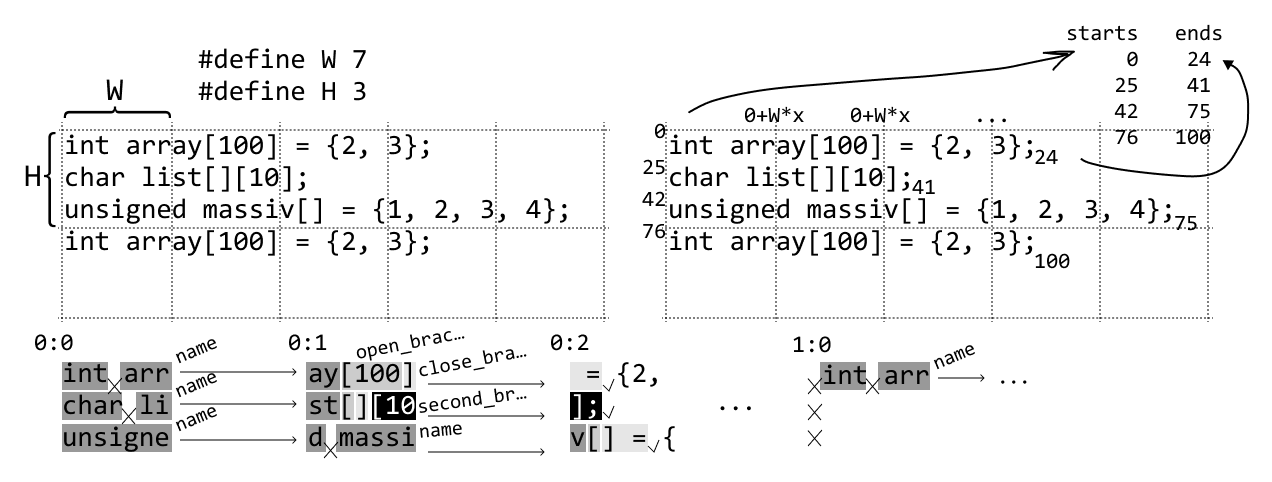
\includegraphics[width=\linewidth]{figures/Frame 12.png}}

Ниже представлены блок-схемы функций (функции стандартного класса, а также функции установки
и получения членов класса, опущены).

\begin{center}
    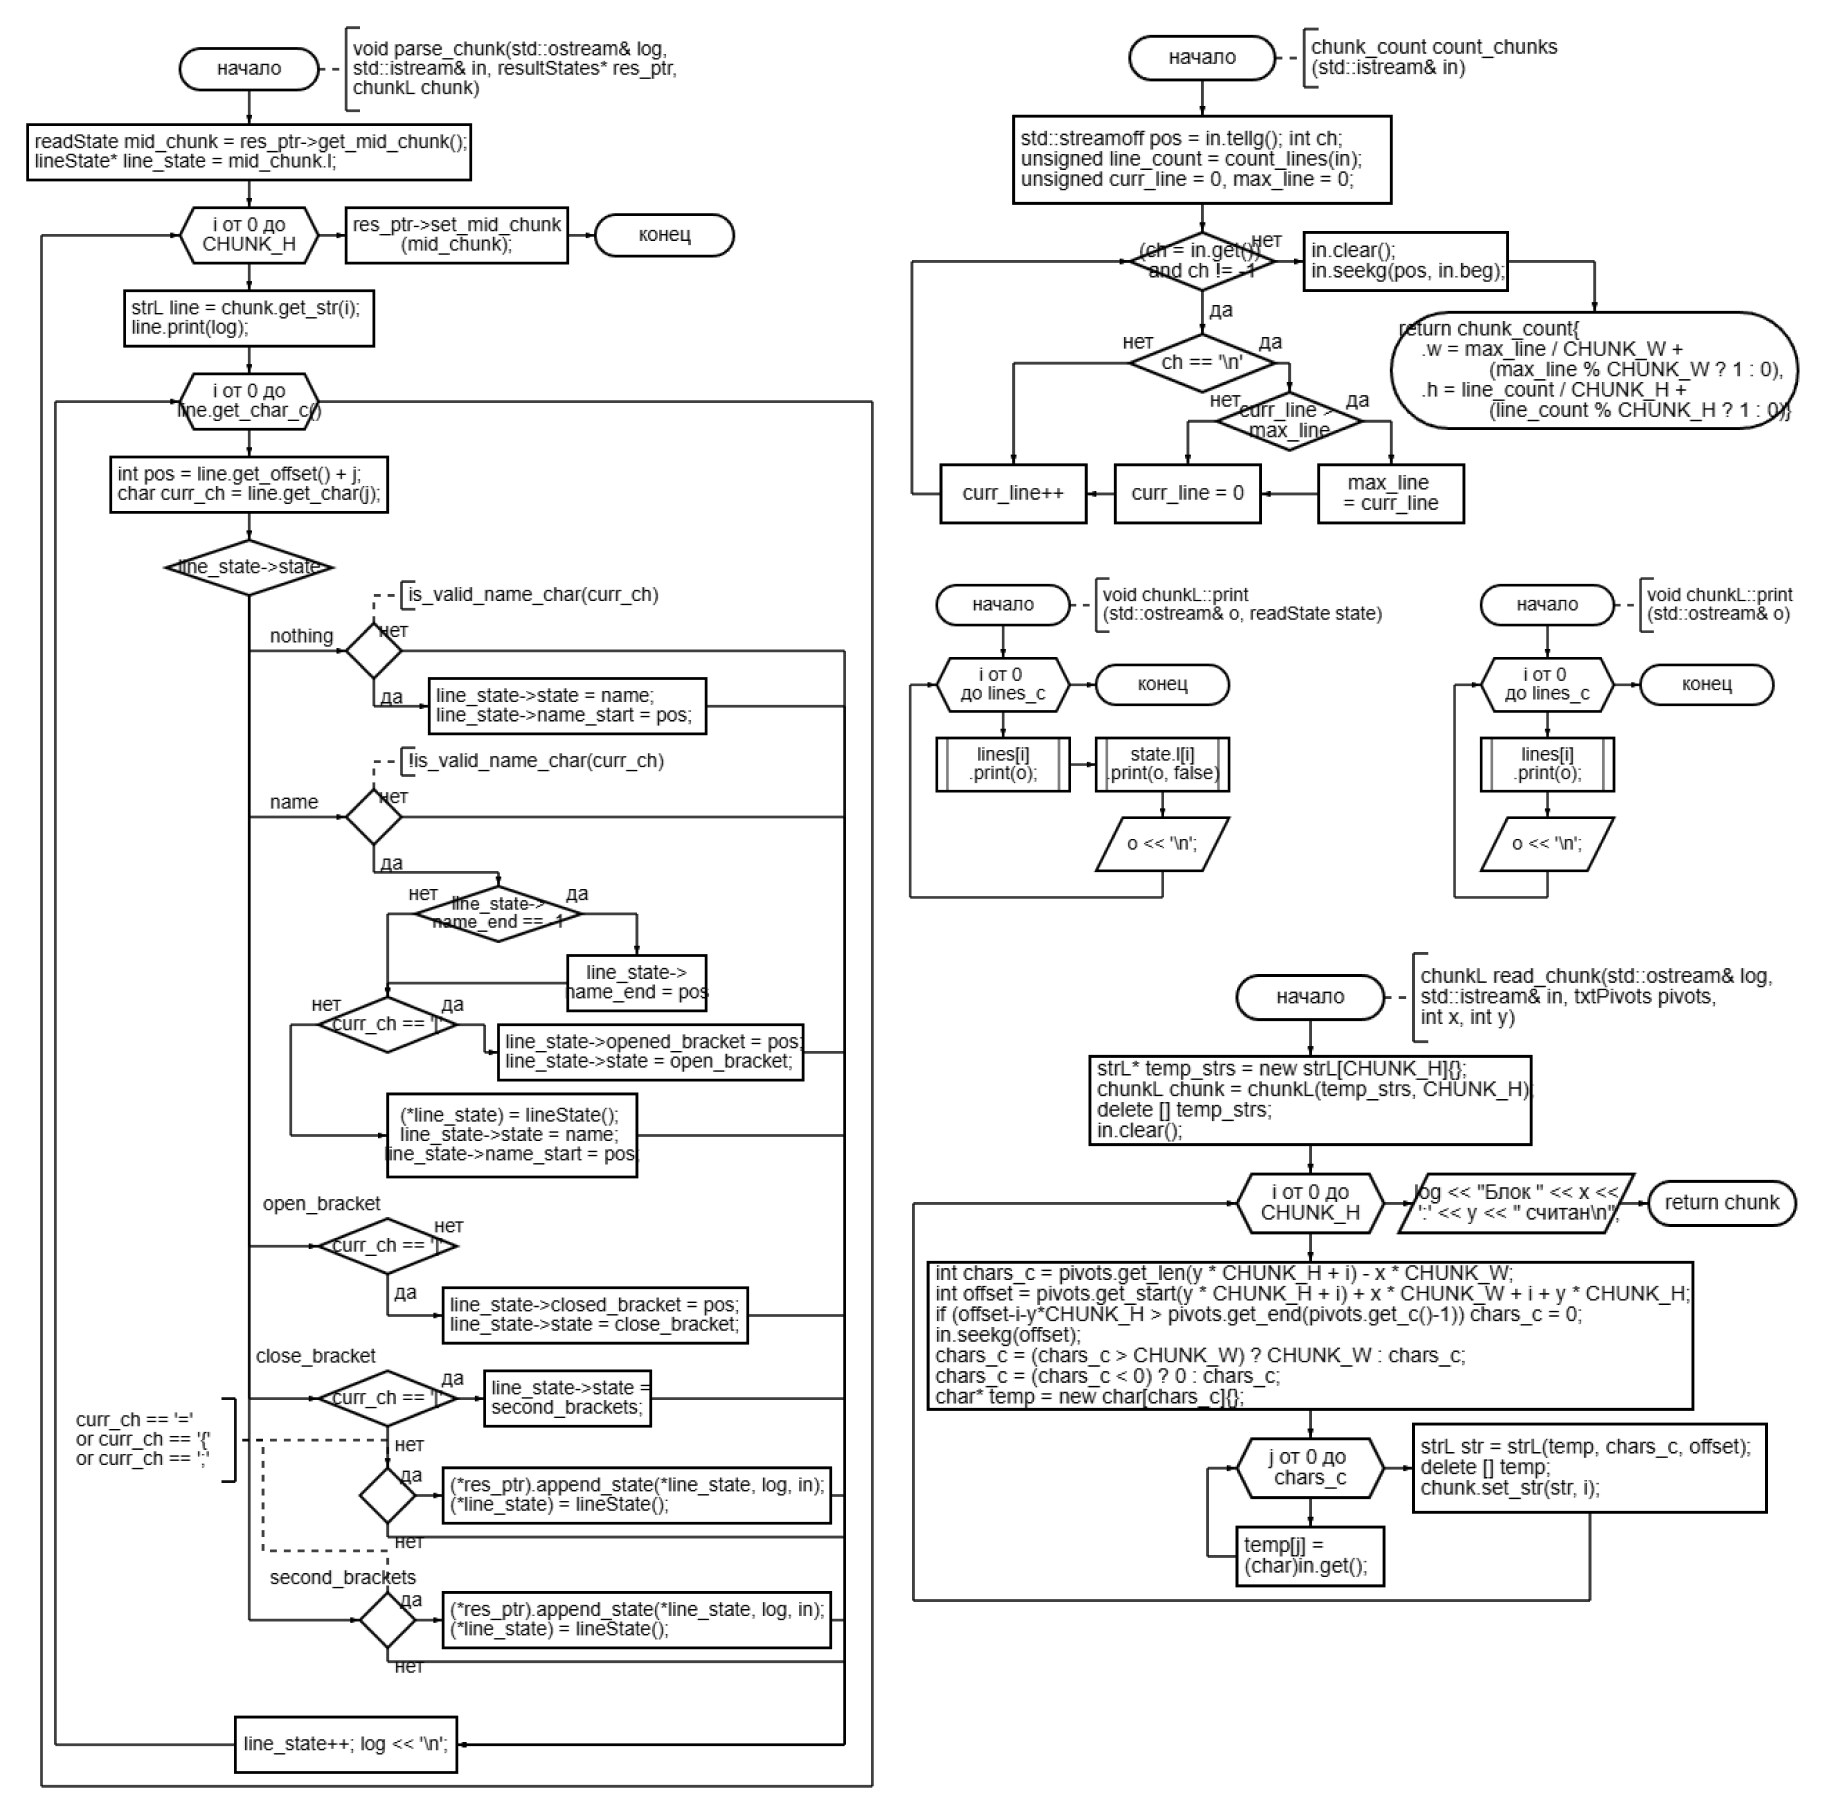
\includegraphics[width=\linewidth]{figures/Frame 13.png}
\end{center}
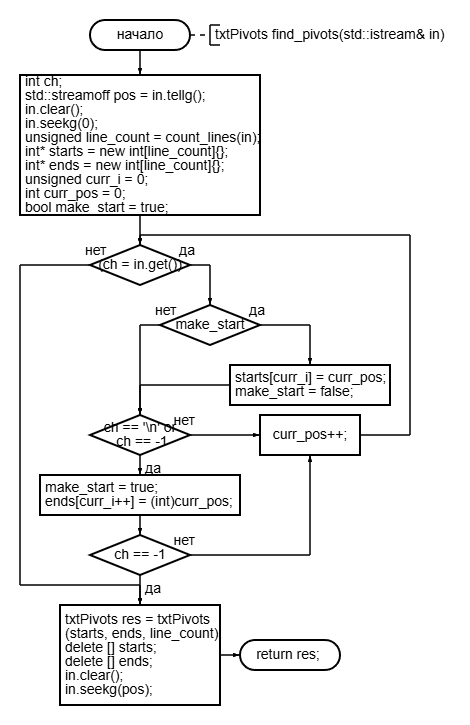
\includegraphics[width=0.4\linewidth]{figures/find_pivots.png}
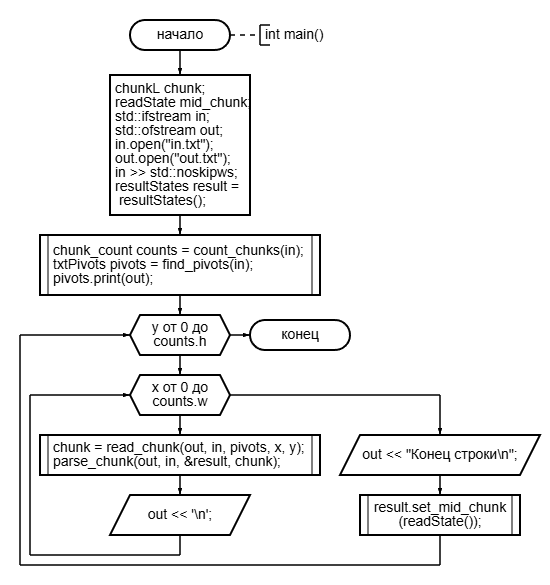
\includegraphics[width=0.4\linewidth]{figures/main.png}

\section{Исходный код программы}

\begin{xltabular}
    {\textwidth}{X|X}
    strL.hpp: \lstinputlisting[language=C++]{../../tasks/2/modules/strL.hpp} &
    strL.cpp: \lstinputlisting[language=C++]{../../tasks/2/modules/strL.cpp} \\
    chunkL.hpp: \lstinputlisting[language=C++]{../../tasks/2/modules/chunkL.hpp} &
    chunkL.cpp: \lstinputlisting[language=C++, lastline=47]{../../tasks/2/modules/chunkL.cpp} \\
\end{xltabular}

\lstinputlisting[language=C++, firstline=48, lastline=167]{../../tasks/2/modules/chunkL.cpp}

\begin{xltabular}
    {\textwidth}{X|X}
    files.hpp: \lstinputlisting[language=C++]{../../tasks/2/modules/files.hpp} &
    files.cpp: \lstinputlisting[language=C++, lastline=34]{../../tasks/2/modules/files.cpp} \\
\end{xltabular}
\lstinputlisting[language=C++, firstline=35]{../../tasks/2/modules/files.cpp}
\begin{xltabular}
    {\textwidth}{X|X}
    readState.hpp: \lstinputlisting[language=C++]{../../tasks/2/modules/readState.hpp} &
    readState.cpp: \lstinputlisting[language=C++, lastline=34]{../../tasks/2/modules/readState.cpp} \\
\end{xltabular}
\lstinputlisting[language=C++]{../../tasks/2/main.cpp}

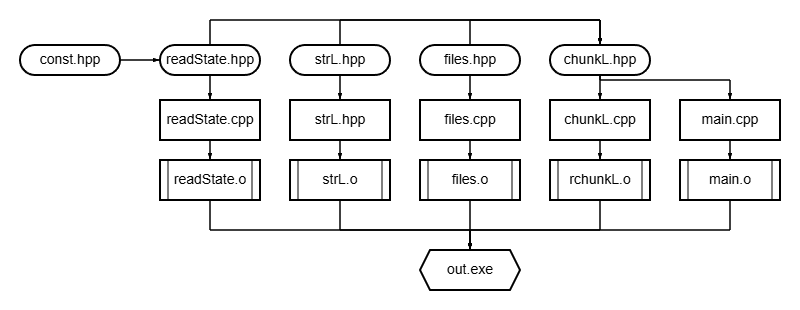
\includegraphics[width=\textwidth]{figures/module_diagram.png}

\section{Результаты работы программы}
\begin{tabularx}{\textwidth}{|>{\ttfamily\footnotesize}X|>{\ttfamily\footnotesize}X|}
    \hline
    \multicolumn{2}{|X|}{Ввод} \\ \hline
    \multicolumn{2}{|X|}{\lstinputlisting{../../tasks/2/in.txt}} \\ \hline
    \multicolumn{2}{|X|}{Вывод} \\ \hline
    \lstinputlisting{out1.txt} & \lstinputlisting{out2.txt} \\ \hline
\end{tabularx}

\section{Вывод о проделанной работе}
В ходе выполнения работы я научился интересному способу чтения из файла, блочному представлению, а также рассмотрел
отличительные особенности массивов, как синтаксических структур.

\end{document}
